\subsection{HTTP Server/Express \texttt{SocketContext}}

\begin{frame}{HTTP Server/Express \texttt{SocketContext}}{Application Protocols}
  \begin{center}
    \begin{figure}
      \par\bigskip
      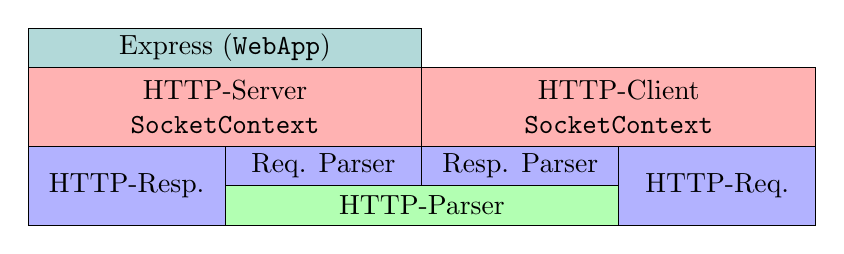
\begin{tikzpicture}
        \draw node [anchor=south, outer sep=0, inner sep=0, draw, fill=green!30, minimum width=5cm, minimum height=0.5cm] (http-p) {HTTP-Parser};

        \draw (http-p.south west) node[anchor=south east, outer sep=0, inner sep=0, draw, fill=blue!30, minimum width=2.5cm, minimum height=1cm] (http-res) {HTTP-Resp.};

        \draw (http-p.south east) node[anchor=south west, outer sep=0, inner sep=0, draw, fill=blue!30, minimum width=2.5cm, minimum height=1cm] (http-res) {HTTP-Req.};

        \draw (http-p.north west) node[anchor=south west, outer sep=0, inner sep=0, draw, fill=blue!30, minimum width=2.5cm, minimum height=0.5cm] (http-reqp) {Req. Parser};

        \draw (http-p.north east) node[anchor=south east, outer sep=0, inner sep=0, draw, fill=blue!30, minimum width=2.5cm, minimum height=0.5cm] (http-respp) {Resp. Parser};

        \draw (http-respp.north west) node[outer sep=0, inner sep=0, anchor=south west, fill=red!30, draw, minimum width=5cm, minimum height=1cm, align=center] (http-c) {HTTP-Client\\\texttt{SocketContext}};

        \draw (http-reqp.north east) node[outer sep=0, inner sep=0, anchor=south east, fill=red!30, draw, minimum width=5cm, minimum height=1cm, align=center] (http-s) {HTTP-Server\\\texttt{SocketContext}};

        \draw (http-s.north) node[anchor=south, draw, fill=teal!30, outer sep=0, inner sep=0, minimum height=0.5cm, minimum width=5cm] (ex) {Express (\texttt{WebApp})};
      \end{tikzpicture}
      \caption{HTTP application protocol layer in detail.}
    \end{figure}
  \end{center}\begin{itemize}
     \item Express is based on the generic HTTP server \texttt{SocketContext} and offers the user an extended API (similar to that of Node.JS/Express).
     \item Express is therefore a sub-framework  (application) of the HTTP server framework.
   \end{itemize}
\end{frame}
